\section{Exercise 3}
\label{sec:ex3}
For the third exercise, we are going to exploit another buffer overflow vulnerability, this time with version \texttt{9.0} of Adobe Reader. We introduce the concept of process migration of the remote shell code, making the exploit execution less visible to the victim.

In order to carry out this attack, we are going to focus on our Windows XP SP2 machine. While at a first glance this might seem like an extremely outdated and pointless attack, in reality \texttt{PDF} files are often the veichle of exploits, even in 2021\footnote{\url{https://threatpost.com/adobe-zero-day-bug-acrobat-reader/166044/}}. First, we will craft our malicious \texttt{PDF} using Metasploit and bundle it into an apparently innocuous file. Then, we will deliver the payload to the target's machine. By the time the victim has opened the file and closed Adobe Reader, we will have full control of his machine.

\subsection{Infected \texttt{PDF} file creation}
\label{subsec:ex3:infected-pdf-file-creation}
The initial phase of the attack in completely handled by \hltexttt{\mbox{msfconsole}}. A set of \hltexttt{\mbox{msfconsole}} scripts are dedicated to the generation of corrupted files, under \texttt{exploit/windows/fileformat/}. This time, we're going to use the \texttt{adobe\_jbig2decode} (Figure \ref{fig:ex3:selecting-exploit}).

\begin{figure}[htbp]
    \centering
    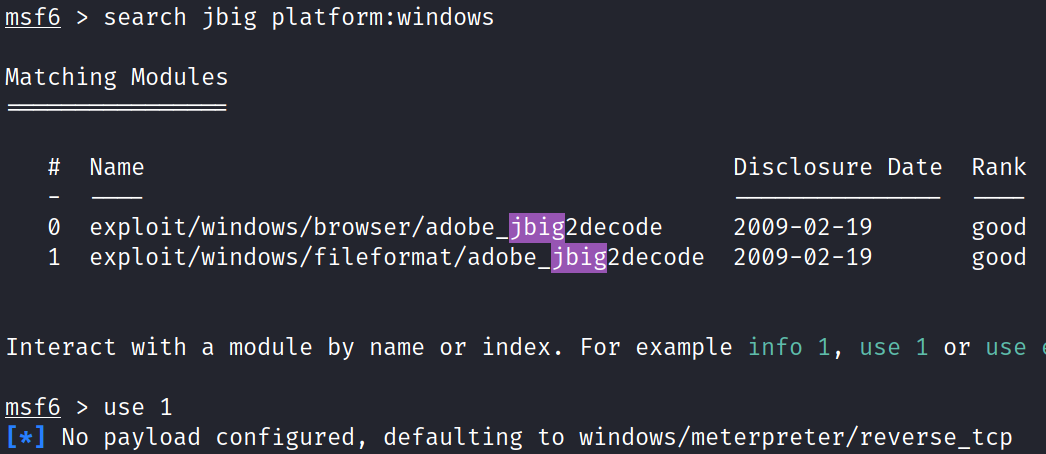
\includegraphics[width=0.7\textwidth]{../drawable/exercise_3_screenshots/module_selection.png}
    \caption{Selecting the exploit to use}
    \label{fig:ex3:selecting-exploit}
\end{figure}

The payload for the infected file will create a reverse shell from the specified host. We set the \texttt{LHOST} and \texttt{LPORT} parameters for binding the shell, and we create the file (Figure \ref{fig:ex3:running-exploit}).

\begin{figure}[htbp]
    \centering
    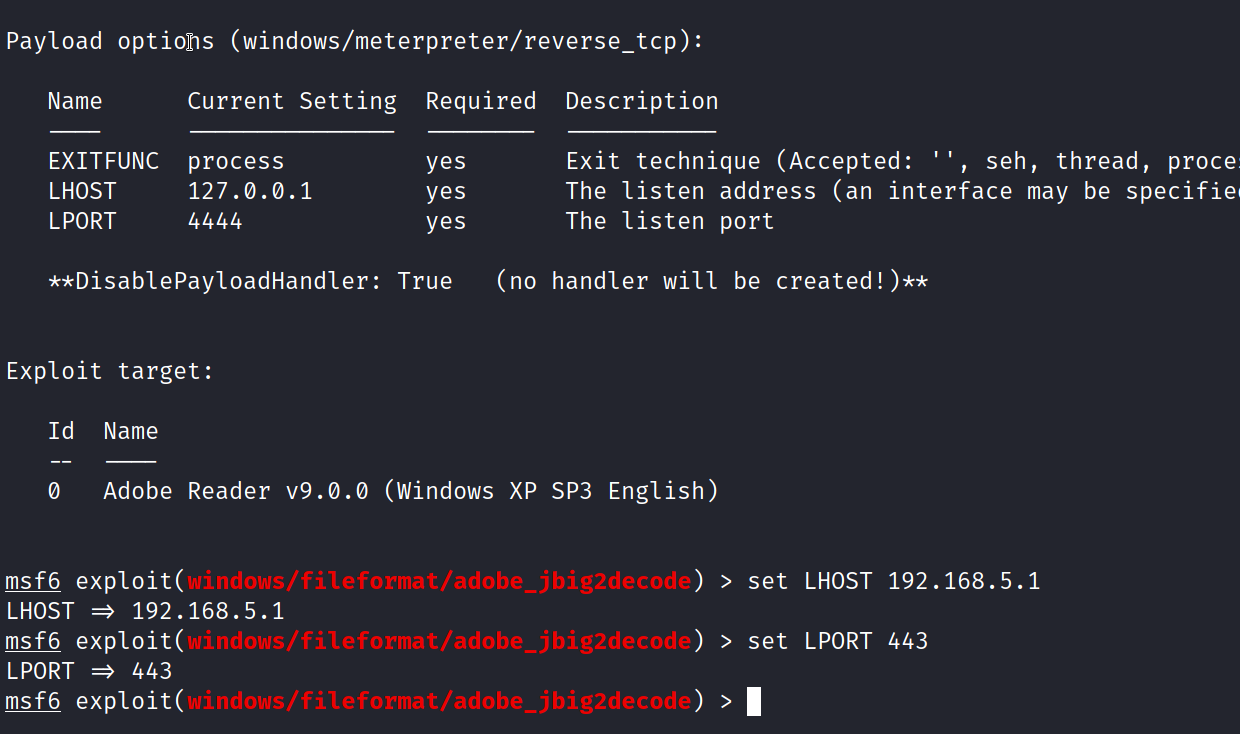
\includegraphics[width=0.7\textwidth]{../drawable/exercise_3_screenshots/module_set_options.png}
    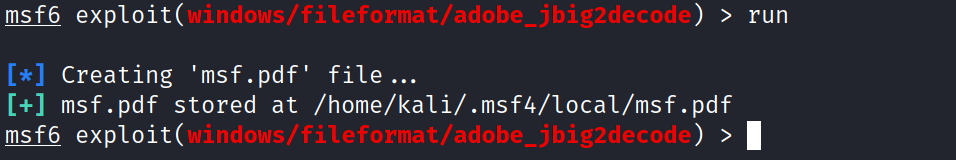
\includegraphics[width=0.7\textwidth]{../drawable/exercise_3_screenshots/run_exploit.png}
    \caption{Setting the options and generating the infected \texttt{PDF}}
    \label{fig:ex3:running-exploit}
\end{figure}

\subsection{Simulated infection}
\label{subsec:ex3:simulated-infection}

In a real life situation, the file could be sent to the victim via email or using a removable media. This is a perfect example on how social engineering could be exploited in conjunction with code-based hacking in order to get even larger footholds in target networks. Moreover, it sends red flags to pentesters who must take care of both automated and well-crafted attacks to the network in their reports.
\begin{figure}[htbp]
    \centering
    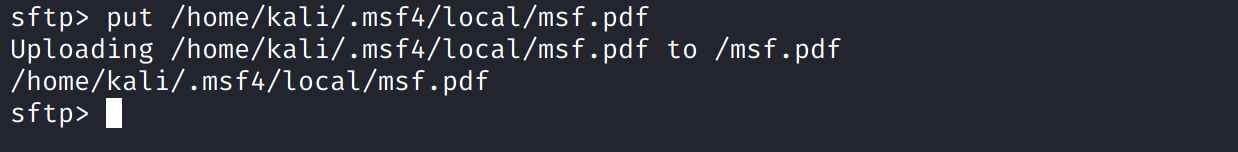
\includegraphics[width=0.7\textwidth]{../drawable/exercise_3_screenshots/put_completed.png}
    \caption{Sending the file to our Windows XP VM}
    \label{fig:ex3:sending-file}
\end{figure}

In this simulation, the file is copied to the victim via \texttt{SFTP}, since in this exercise we are more interested in the effects of the exploit rather than the delivery of the infected file. Figure \ref{fig:ex3:sending-file} shows the sending of the file. Notice that an \texttt{SFTP} server was previously installed on the Windows XP machine, listening on port \texttt{22}, as \texttt{SFTP} runs on the \texttt{SSH} port instead of the regular \texttt{FTP} ones. That port was the only one appearing as open in the results of the scans in Sections \ref{sec:exercise1:tcpscanning} and \ref{subsec:ex2:scanning-again}.

\subsection{Reverse shell handler}
\label{subsec:ex3:reverse-shell-handler}

Differently from the previous exercise, the reverse shell handler needs to be started manually (Figure \ref{fig:ex3:reverse-shell-handler}). This is because the previous exploit was "just" limited to the creation of the malicious file and did not provide an automatic connection feature. However, we can quickly take care of this problem.

\begin{figure}[htbp]
    \centering
    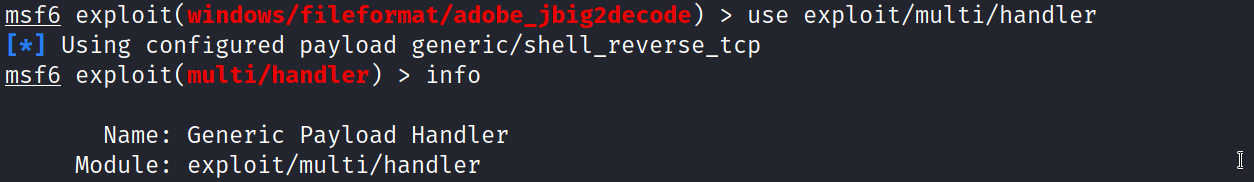
\includegraphics[width=0.7\textwidth]{../drawable/exercise_3_screenshots/generic_payload_handler.png}
    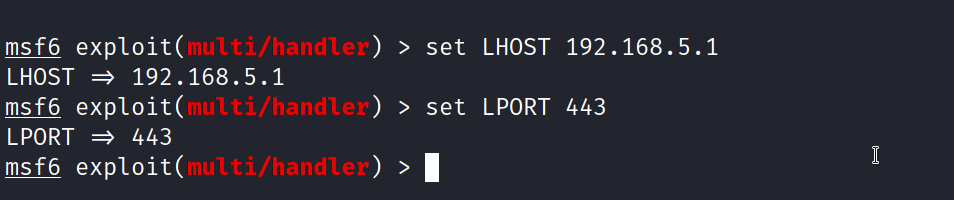
\includegraphics[width=0.7\textwidth]{../drawable/exercise_3_screenshots/set_handler_parameters.png}
    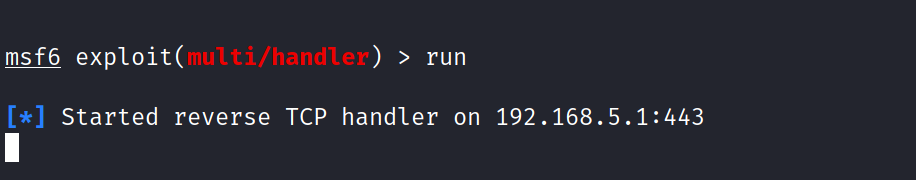
\includegraphics[width=0.7\textwidth]{../drawable/exercise_3_screenshots/handler_listening.png}
    \caption{Starting the reverse shell handler}
    \label{fig:ex3:reverse-shell-handler}
\end{figure}

When the victim opens the \texttt{PDF} file, the exploit code causes a buffer overflow, and redirects the execution of the Adobe Reader process towards the code of our payload. The payload contacts the attacker on port \texttt{443} (port for \texttt{HTTPS} service); using well-known ports allows us to bypass the victim's host firewall. Figure \ref{fig:ex3:reverse-shell-opened} shows a successfully open shell.

\begin{figure}[htbp]
    \centering
    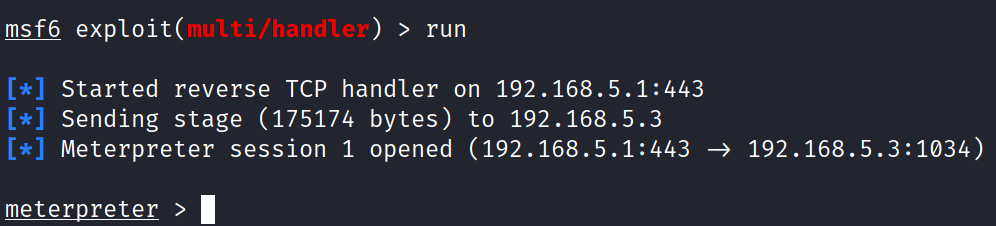
\includegraphics[width=0.7\textwidth]{../drawable/exercise_3_screenshots/meterpreter_opened.png}
    \caption{Reverse shell managed to reach the attacker}
    \label{fig:ex3:reverse-shell-opened}
\end{figure}

\subsection{Exploit code migration}
\label{subsec:ex3:exploit-code-migration}

After the victim has opened the file, Adobe Reader freezes. This may prompt the user to forcefully kill the viewer, thus terminating our reverse shell. To avoid this, we can use a standard functionality of the Meterpreter console to migrate the code of the reverse shell to another process. Figure \ref{fig:ex3:migrating-shell} shows this process.

\begin{figure}[htbp]
    \centering
    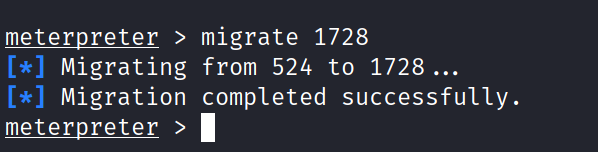
\includegraphics[width=0.7\textwidth]{../drawable/exercise_3_screenshots/meterpreter_migration.png}
    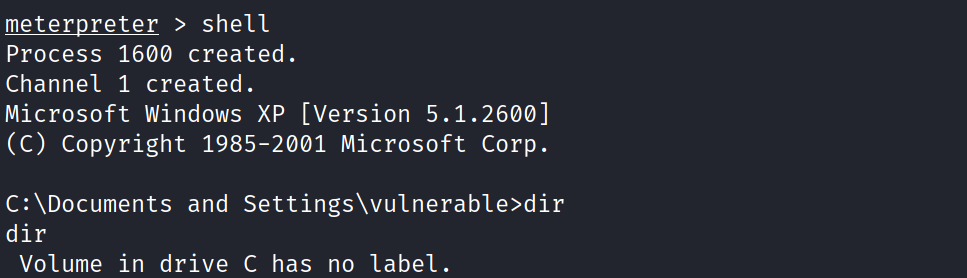
\includegraphics[width=0.7\textwidth]{../drawable/exercise_3_screenshots/meterpreter_shell_opened_cropped.png}
    \caption{Migrating shell code to another process}
    \label{fig:ex3:migrating-shell}
\end{figure}

This works because Windows allows to write data into a process memory, allowing to "hot patch" the code of a process with our exploit. When the migration completes, the reverse shell remains active even if the victim kills the Adobe Reader process.

\subsection{Exploit details}
\label{subsec:ex3:exploit-details}
 The exploit used in this exercise is \texttt{CVE-2009-0658}: 
\medskip
\begin{center}
\noindent\fbox{%
    \parbox{0.9\textwidth}{%
    Buffer overflow in Adobe Reader 9.0 and earlier, and Acrobat 9.0 and earlier, allows remote attackers to execute arbitrary code via a crafted \texttt{PDF} document, related to a non-JavaScript function call and possibly an embedded JBIG2 image stream, as exploited in the wild in February 2009 by \texttt{Trojan.Pidief.E}.        
    }%
}
\end{center}
\medskip

The attack is not completely invisible to the target. Tools like \texttt{netstat} can see the connection towards the attacker. Depending on the situation, the user may or may not be capable of using such tools during their daily work usage. Either way, targeting a less tech savy user would be the wisest choice here.

\begin{figure}[htbp]
    \centering
    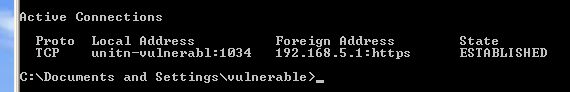
\includegraphics[width=0.75\textwidth]{../drawable/exercise_3_screenshots/victim_connection.PNG}
    \caption{Output of \texttt{netstat} on victim machine while the payload executes}
    \label{fig:ex3:victim-connections}
\end{figure}

\clearpage